\documentclass[12pt,a4paper]{article}

\usepackage[a4paper,margin=1in]{geometry}
\usepackage{fontspec}
\usepackage{setspace}
\usepackage{amsmath,amssymb}
\usepackage{booktabs}
\usepackage{array}
\usepackage{enumitem}
\usepackage{microtype}
\usepackage{tikz}
\usepackage{xcolor}
\usepackage{hyperref}
\usetikzlibrary{arrows.meta,positioning,shapes.geometric}

\setmainfont{Times New Roman}
\singlespacing
\setlength{\parindent}{1.5em}
\setlength{\parskip}{0pt}
\setlist{nosep,leftmargin=1.8em}
\setcounter{secnumdepth}{2}
\pagestyle{plain}

\definecolor{farblue}{HTML}{2F6B9A}
\definecolor{nearorange}{HTML}{C56A22}
\definecolor{softgray}{HTML}{F1F3F5}
\definecolor{darkgreen}{HTML}{347A57}

\hypersetup{
  colorlinks=true,
  linkcolor=black,
  citecolor=black,
  urlcolor=farblue,
  pdftitle={Channel Estimation for XL-MIMO: Final Report},
  pdfauthor={Student Name}
}

\newcommand{\fieldvec}[1]{\boldsymbol{#1}}
\newcommand{\tightsection}[1]{\section{#1}\vspace{-0.35em}}
\newcommand{\infofield}[2]{\textbf{#1:} #2\hfill}

\begin{document}

% ---------------------------------------------------------------------------
% Page 1: Introduction and contributions
% ---------------------------------------------------------------------------
\begin{center}
  {\Large\bfseries Channel Estimation for Extremely Large-Scale Massive
  MIMO:\\[0.15em] Far-Field, Near-Field, or Hybrid-Field?}

  \vspace{0.55em}
  \infofield{Course}{{Principles of Wireless Communications}}\\[0.35em]
  \infofield{Student}{朱昱安、何傳盛、楊予綸、柯均儒、陳楷寰、王郁仁}\\[0.35em]
  \infofield{Instructor}{Prof. Shih-Chun Lin}
  \infofield{Date}{2026/06/09}
\end{center}

\vspace{-0.5em}
\tightsection{Introduction}

Extremely large-scale massive multiple-input multiple-output (XL-MIMO)
equips a base station (BS) with hundreds of antennas. The resulting aperture
offers high array gain and spatial resolution for future 6G systems, but it
also creates a difficult channel-estimation problem: the channel dimension
grows with the antenna count, while sending one orthogonal pilot per antenna
would consume an impractical amount of time and spectrum.

Wei and Dai identify a second problem that is specific to very large
apertures \cite{wei2022}. Conventional massive-MIMO estimation assumes that
all relevant scatterers are far from the array, so their waves are planar.
In XL-MIMO, the Rayleigh distance can extend tens of metres; nearby
scatterers then produce spherical waves. A practical channel can therefore
contain far-field and near-field paths at the same time. The paper calls
this the \emph{hybrid-field} condition.

\begin{figure}[ht]
  \centering
  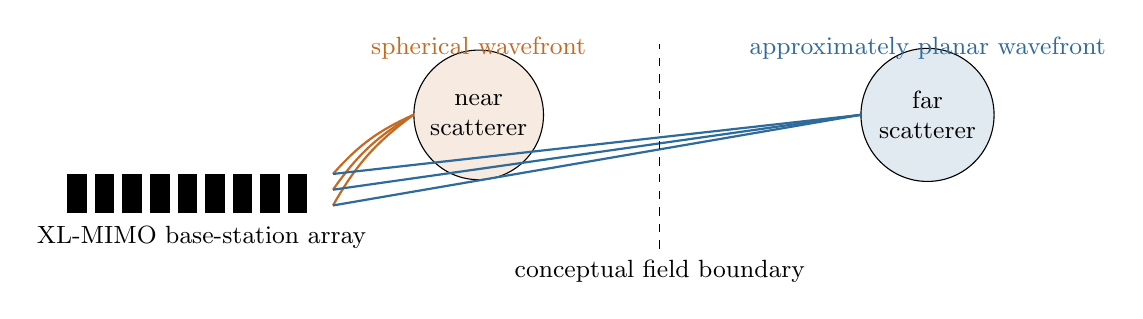
\begin{tikzpicture}[
      >=Latex,
      antenna/.style={draw,fill=black,minimum width=0.08cm,minimum height=0.48cm},
      scatter/.style={circle,draw,minimum size=0.56cm,align=center,font=\small},
      label/.style={font=\small,align=center}
    ]
    \foreach \x in {0,0.35,...,3.15}
      \node[antenna] at (\x,0) {};
    \node[label] at (1.58,-0.55) {XL-MIMO base-station array};

    \node[scatter,fill=nearorange!14] (near) at (5.1,1.0) {near\\scatterer};
    \node[scatter,fill=farblue!14] (far) at (10.8,1.0) {far\\scatterer};
    \node[label,nearorange] at (5.1,1.85) {spherical wavefront};
    \node[label,farblue] at (10.8,1.85) {approximately planar wavefront};

    \foreach \y in {-0.15,0.05,0.25}
      \draw[nearorange,thick] (3.25,\y) to[bend left=12] (near.west);
    \foreach \y in {-0.15,0.05,0.25}
      \draw[farblue,thick] (3.25,\y) -- (far.west);
    \draw[dashed] (7.4,-0.7) -- (7.4,1.9);
    \node[label] at (7.4,-0.98) {conceptual field boundary};
  \end{tikzpicture}
  \caption{Original conceptual illustration of a hybrid-field XL-MIMO
  environment. Different paths can obey different wavefront models.}
  \label{fig:environment}
\end{figure}

\tightsection{Problem and Contributions}

Far-field methods exploit sparsity in an angle-domain dictionary, whereas
near-field methods use a larger polar-domain dictionary indexed by angle
and distance. Applying either one to the complete hybrid channel produces
model mismatch and energy leakage. The paper addresses this gap through
three linked contributions:
\begin{enumerate}
  \item It identifies mixed far-field and near-field propagation as a
  realistic XL-MIMO channel feature.
  \item It introduces a hybrid-field model whose mixing parameter controls
  the proportion of the two path types.
  \item It proposes hybrid-field orthogonal matching pursuit (HF-OMP),
  which estimates each path type in its matching sparse domain while
  retaining low pilot overhead.
\end{enumerate}

\newpage

% ---------------------------------------------------------------------------
% Page 2: System and existing models
% ---------------------------------------------------------------------------
\tightsection{Signal Model and Propagation Regions}

For downlink training from an $N$-antenna BS to a single-antenna user, the
received pilots are
\begin{equation}
  \fieldvec{y}=\fieldvec{P}\fieldvec{h}+\fieldvec{n},
  \label{eq:signal}
\end{equation}
where $\fieldvec{h}$ is the channel, $\fieldvec{P}$ is the pilot matrix,
and $\fieldvec{n}$ is noise. Since low-overhead estimation requires
$M\ll N$, recovery depends on a sparse physical model.

The boundary between propagation regions is approximated by the Rayleigh
distance
\begin{equation}
  Z=\frac{2D^{2}}{\lambda},
  \label{eq:rayleigh}
\end{equation}
with aperture $D$ and wavelength $\lambda$. Scatterers beyond $Z$ use a
planar-wave model; those inside $Z$ require a spherical-wave model. Because
$Z$ grows quadratically with $D$, XL-MIMO greatly enlarges the near field.

\tightsection{Existing Sparse Channel Models}

\subsection{Far-Field: Angle-Domain Sparsity}

For $L$ paths, planar-wave phases progress linearly across the array. The
channel is represented as
\begin{equation}
  \fieldvec{h}_{\mathrm{far}}=\fieldvec{F}\fieldvec{h}^{A},
  \label{eq:far}
\end{equation}
where $\fieldvec{F}$ is a DFT dictionary and $\fieldvec{h}^{A}$ is sparse
because only a few angles contain paths. Angle-domain OMP exploits this
sparsity.

\subsection{Near-Field: Polar-Domain Sparsity}

A spherical wave depends on angle and distance, so a DFT dictionary spreads
its energy across many bins. The polar representation is
\begin{equation}
  \fieldvec{h}_{\mathrm{near}}=\fieldvec{W}\fieldvec{h}^{P},
  \label{eq:near}
\end{equation}
where $\fieldvec{W}$ samples angle--distance points and
$\fieldvec{h}^{P}$ is sparse. It is accurate for nearby scatterers, but
$\fieldvec{W}$ is larger and less orthogonal than $\fieldvec{F}$.

\begin{table}[!ht]
  \centering
  \caption{Comparison of the two conventional models.}
  \label{tab:models}
  \small
  \renewcommand{\arraystretch}{0.98}
  \begin{tabular}{>{\raggedright\arraybackslash}p{2.2cm}
                  >{\raggedright\arraybackslash}p{2.8cm}
                  >{\raggedright\arraybackslash}p{2.8cm}
                  >{\raggedright\arraybackslash}p{3.2cm}}
    \toprule
    & \textbf{Far field} & \textbf{Near field} & \textbf{Mismatch effect} \\
    \midrule
    Wavefront & Planar & Spherical & Phase mismatch \\
    Variables & Angle & Angle and distance & Energy spread \\
    Sparse domain & DFT/angle & Polar & Extra atoms \\
    Dictionary & $N\times N$ & $N\times S$, $S>N$ & Coherence and cost \\
    \bottomrule
  \end{tabular}
\end{table}

For a mixed channel, near-field paths leak in $\fieldvec{F}$ and far-field
paths leak in $\fieldvec{W}$. The complete channel is therefore not sparse
enough in either single dictionary for accurate conventional OMP.

\newpage

% ---------------------------------------------------------------------------
% Page 3: Hybrid-field model
% ---------------------------------------------------------------------------
\tightsection{Proposed Hybrid-Field Channel Model}

The paper models the channel as a superposition of far-field and near-field
components:
\begin{equation}
\begin{split}
  \fieldvec{h}_{\mathrm{hybrid}}
  ={}& \sqrt{\frac{N}{L}}
  \sum_{\ell_f=1}^{\gamma L}
    \alpha_{\ell_f}\fieldvec{a}(\theta_{\ell_f})\\
  &+\sqrt{\frac{N}{L}}
  \sum_{\ell_n=1}^{(1-\gamma)L}
    \beta_{\ell_n}\fieldvec{b}(\theta_{\ell_n},r_{\ell_n}),
\end{split}
\label{eq:hybrid}
\end{equation}
where $L$ is the total number of paths and $\gamma\in[0,1]$ controls their
composition. The first sum contains $\gamma L$ planar-wave paths, and the
second contains $(1-\gamma)L$ spherical-wave paths.

This formulation is general rather than a third unrelated propagation
law. At $\gamma=1$, it reduces to the standard far-field model. At
$\gamma=0$, it becomes the near-field model. Intermediate values describe
mixed environments, such as a distant direct link accompanied by
scatterers close to the BS.

\begin{figure}[ht]
  \centering
  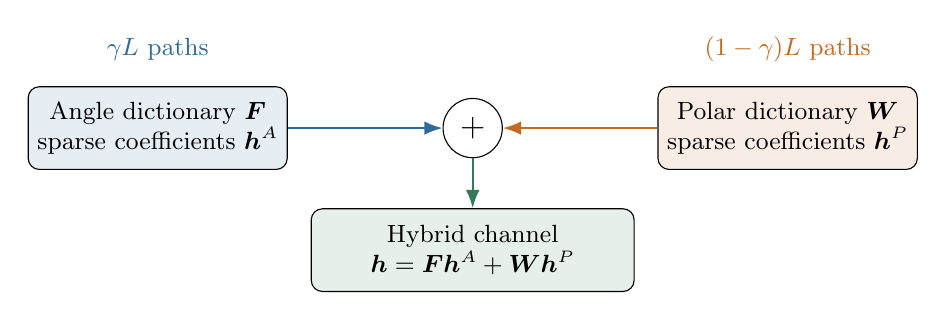
\begin{tikzpicture}[
      >=Latex,
      box/.style={draw,rounded corners,minimum width=3.2cm,minimum height=1.05cm,
                  align=center,font=\small},
      plus/.style={circle,draw,minimum size=0.62cm,font=\large},
      note/.style={font=\small,align=center}
    ]
    \node[box,fill=farblue!12] (far) at (0,0)
      {Angle dictionary $\fieldvec{F}$\\sparse coefficients $\fieldvec{h}^{A}$};
    \node[plus] (plus) at (4.0,0) {$+$};
    \node[box,fill=nearorange!12] (near) at (8.0,0)
      {Polar dictionary $\fieldvec{W}$\\sparse coefficients $\fieldvec{h}^{P}$};
    \node[box,fill=darkgreen!12,minimum width=4.1cm] (hybrid) at (4.0,-1.55)
      {Hybrid channel\\$\fieldvec{h}=\fieldvec{F}\fieldvec{h}^{A}
      +\fieldvec{W}\fieldvec{h}^{P}$};
    \draw[->,thick,farblue] (far) -- (plus);
    \draw[->,thick,nearorange] (near) -- (plus);
    \draw[->,thick,darkgreen] (plus) -- (hybrid);
    \node[note,farblue] at (0,1.0) {$\gamma L$ paths};
    \node[note,nearorange] at (8.0,1.0) {$(1-\gamma)L$ paths};
  \end{tikzpicture}
  \caption{Original representation of the hybrid-field model as the sum of
  two components that are sparse in different dictionaries.}
  \label{fig:representation}
\end{figure}

\tightsection{Why a Single Dictionary Fails}

Substituting the two sparse representations into
Equation~\eqref{eq:signal} gives
\begin{equation}
  \fieldvec{y}
  =\fieldvec{P}\fieldvec{F}\fieldvec{h}^{A}
   +\fieldvec{P}\fieldvec{W}\fieldvec{h}^{P}
   +\fieldvec{n}.
  \label{eq:joint}
\end{equation}
This equation exposes the estimation challenge. If far-field OMP uses only
$\fieldvec{P}\fieldvec{F}$, the spherical-wave component behaves like
structured interference and may require many angle atoms. If near-field
OMP uses only $\fieldvec{P}\fieldvec{W}$, a planar-wave component can leak
among multiple polar atoms. In either case, the assumed sparsity level and
the true representation no longer agree.

\tightsection{Interpretation and Significance}

The main conceptual contribution is to match each physical path class with
its natural coordinate system. The hybrid model preserves the low number
of physical scatterers instead of forcing every path into one oversized
representation. It also provides a controlled simulation framework:
varying $\gamma$ tests pure near-field, mixed-field, and pure far-field
conditions with the same total path count.

HF-OMP assumes that $L$ and $\gamma$ are known. A practical system would
need to estimate or select both values adaptively.

\newpage

% ---------------------------------------------------------------------------
% Page 4: HF-OMP
% ---------------------------------------------------------------------------
\tightsection{HF-OMP Channel Estimation}

HF-OMP separates Equation~\eqref{eq:joint} into two sparse-recovery stages.
It first searches the smaller, better-conditioned angle dictionary and
then explains the remaining observation with the polar dictionary.

\begin{figure}[ht]
  \centering
  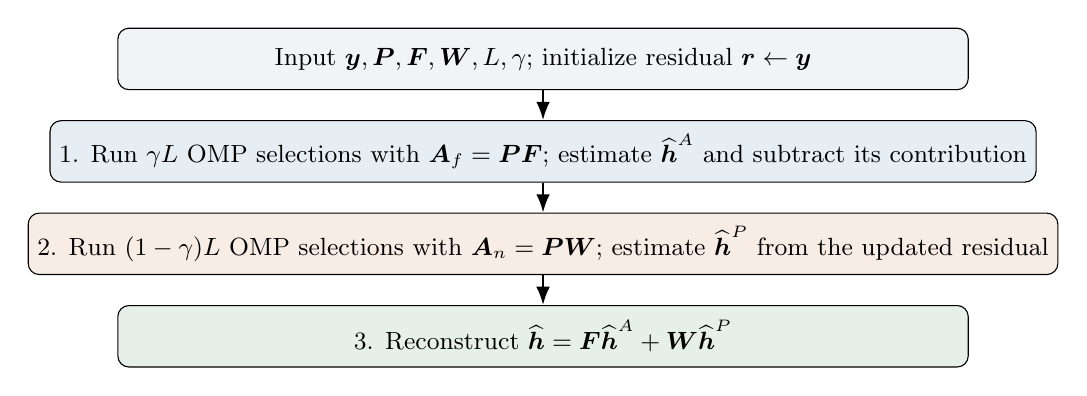
\begin{tikzpicture}[
      >=Latex,
      flowbox/.style={draw,rounded corners,fill=softgray,minimum width=10.8cm,
                   minimum height=0.78cm,align=center,font=\small},
      arrow/.style={->,thick}
    ]
    \node[flowbox] (input) {Input $\fieldvec{y},\fieldvec{P},\fieldvec{F},
      \fieldvec{W},L,\gamma$; initialize residual
      $\fieldvec{r}\leftarrow\fieldvec{y}$};
    \node[flowbox,fill=farblue!12,below=0.38cm of input] (far)
      {1. Run $\gamma L$ OMP selections with
      $\fieldvec{A}_{f}=\fieldvec{P}\fieldvec{F}$; estimate
      $\widehat{\fieldvec{h}}^{A}$ and subtract its contribution};
    \node[flowbox,fill=nearorange!12,below=0.38cm of far] (near)
      {2. Run $(1-\gamma)L$ OMP selections with
      $\fieldvec{A}_{n}=\fieldvec{P}\fieldvec{W}$; estimate
      $\widehat{\fieldvec{h}}^{P}$ from the updated residual};
    \node[flowbox,fill=darkgreen!12,below=0.38cm of near] (out)
      {3. Reconstruct
      $\widehat{\fieldvec{h}}=\fieldvec{F}\widehat{\fieldvec{h}}^{A}
      +\fieldvec{W}\widehat{\fieldvec{h}}^{P}$};
    \draw[arrow] (input) -- (far);
    \draw[arrow] (far) -- (near);
    \draw[arrow] (near) -- (out);
  \end{tikzpicture}
  \caption{Original flowchart of the three-stage HF-OMP procedure.}
  \label{fig:hfomp}
\end{figure}

\subsection{Stage 1: Far-Field Recovery}

With $\fieldvec{A}_{f}=\fieldvec{P}\fieldvec{F}$, each OMP iteration
selects the column most correlated with the current residual. A
least-squares update estimates the gains on the selected support. After
$\gamma L$ selections, the algorithm subtracts the reconstructed far-field
contribution. Starting with this stage is computationally attractive
because $\fieldvec{F}$ has only $N$ orthogonal columns.

\subsection{Stage 2: Near-Field Recovery}

The remaining residual is searched using
$\fieldvec{A}_{n}=\fieldvec{P}\fieldvec{W}$. The selected polar atoms
identify both angle and distance. The residual update accounts for the
estimated near-field component as well as the far-field component already
found. At $\gamma=1$ this stage disappears; at $\gamma=0$ the first stage
disappears, so conventional far-field and near-field OMP are endpoint
cases of HF-OMP.

\subsection{Stage 3: Reconstruction and Complexity}

The two estimated sparse vectors are transformed back to the antenna
domain and added. Following the paper's notation, the approximate
complexity is
\begin{equation}
  \mathcal{O}\!\left(NM(\gamma L)^3\right)
  +\mathcal{O}\!\left(SM((1-\gamma)L)^3\right)
  +\mathcal{O}(NS).
  \label{eq:complexity}
\end{equation}
The polar search is the expensive part because $S$ can greatly exceed
$N$. HF-OMP nevertheless avoids using the large polar dictionary for paths
that are naturally represented by the DFT dictionary.

\tightsection{Practical Trade-Offs}

The sequential structure is simple and interpretable, but early support
errors can contaminate the residual used in Stage 2. Grid-based
dictionaries also create off-grid leakage, and closely spaced atoms in
$\fieldvec{W}$ can be difficult to distinguish. Joint recovery, adaptive
field classification, or off-grid refinement could improve robustness at
the price of additional computation.

\newpage

% ---------------------------------------------------------------------------
% Page 5: Results, assessment, conclusion, references
% ---------------------------------------------------------------------------
\tightsection{Simulation Results}

The simulations use the parameters in Table~\ref{tab:simulation}. With
$M=256<N=512$, the compressed-sensing schemes use half as many pilots as
the MMSE benchmark ($M=512$). HF-OMP is compared with far-field OMP,
near-field OMP, and this full-dimensional benchmark.

\begin{table}[ht]
  \centering
  \caption{Principal simulation settings reported by Wei and Dai.}
  \label{tab:simulation}
  \renewcommand{\arraystretch}{1.1}
  \begin{tabular}{ll@{\qquad}ll}
    \toprule
    BS antennas & $N=512$ & Carrier frequency & $30$ GHz \\
    Wavelength & $\lambda=0.01$ m & Physical paths & $L=6$ \\
    CS pilots & $M=256$ & Polar grid size & $S=2071$ \\
    Path angle & uniform & Path distance & $10$--$80$ m \\
    \bottomrule
  \end{tabular}
\end{table}

\subsection{NMSE versus SNR}

For $\gamma=0.5$, HF-OMP achieves lower normalized mean-square error
(NMSE) than either mismatched OMP baseline across the reported SNR range.
Far-field OMP spreads spherical paths, while near-field OMP represents
planar paths with a coherent, oversized dictionary. HF-OMP improves
accuracy by recovering each component in its sparse domain. The MMSE curve
is not a like-for-like low-overhead method because it uses twice as many
pilots.

\subsection{NMSE versus Field Composition}

At 5 dB, the authors vary $\gamma$. HF-OMP matches near-field OMP at
$\gamma=0$ and far-field OMP at $\gamma=1$, because those are its two
endpoint cases. For mixed channels it performs better than either
single-field estimator. Thus performance depends on modeling field
composition, not only on the sparse-recovery algorithm.

\tightsection{Critical Assessment and Conclusion}

The hybrid model clearly exposes mismatch loss, and HF-OMP adds an
interpretable two-stage search to standard OMP. Its limitations are the
assumptions of known $L$ and $\gamma$, on-grid paths, and a limited
simulation study. The large polar dictionary raises memory and computation,
while far-first recovery can propagate errors.

The paper establishes that XL-MIMO should not be forced into one field
model: domain-matched recovery improves NMSE at the same low pilot
overhead. Future work should estimate $\gamma$, refine off-grid parameters,
use joint or Bayesian recovery, and test wideband, multi-user, and measured
channels.

\renewcommand{\refname}{References}
\begin{thebibliography}{2}
\setlength{\itemsep}{0pt}
\setlength{\parskip}{0pt}
\small

\bibitem{wei2022}
X. Wei and L. Dai, ``Channel estimation for extremely large-scale massive
MIMO: Far-field, near-field, or hybrid-field?'' \emph{IEEE Communications
Letters}, vol. 26, no. 1, pp. 177--181, Jan. 2022,
doi: 10.1109/LCOMM.2021.3124927.

\bibitem{cui2022}
M. Cui and L. Dai, ``Channel estimation for extremely large-scale MIMO:
Far-field or near-field?'' \emph{IEEE Transactions on Communications},
vol. 70, no. 4, pp. 2663--2677, Apr. 2022.

\end{thebibliography}

\newpage

% ---------------------------------------------------------------------------
% Page 6: reserved Q&A
% ---------------------------------------------------------------------------
\section*{Q\&A}
\addcontentsline{toc}{section}{Q\&A}

\noindent
\textit{This page is reserved for questions and answers. Replace the
placeholders below when the final Q\&A content is available.}

\vspace{1.2em}

\noindent\textbf{Question 1.} \rule{0.78\textwidth}{0.4pt}

\vspace{0.7em}
\noindent\textbf{Answer.}\\[0.35em]
\rule{\textwidth}{0.4pt}\\[1.05em]
\rule{\textwidth}{0.4pt}\\[1.05em]
\rule{\textwidth}{0.4pt}

\vspace{1.5em}

\noindent\textbf{Question 2.} \rule{0.78\textwidth}{0.4pt}

\vspace{0.7em}
\noindent\textbf{Answer.}\\[0.35em]
\rule{\textwidth}{0.4pt}\\[1.05em]
\rule{\textwidth}{0.4pt}\\[1.05em]
\rule{\textwidth}{0.4pt}

\vspace{1.5em}

\noindent\textbf{Question 3.} \rule{0.78\textwidth}{0.4pt}

\vspace{0.7em}
\noindent\textbf{Answer.}\\[0.35em]
\rule{\textwidth}{0.4pt}\\[1.05em]
\rule{\textwidth}{0.4pt}\\[1.05em]
\rule{\textwidth}{0.4pt}

\vfill
\begin{center}
  \textit{Additional questions may be added while retaining this page as
  the final section of the report.}
\end{center}

\end{document}
